\chapter{Discussion and Conclusion} \label{sec:discussion_and_conclusion}
    \newpage
    
    \longsection{Introduction}{sec:discussion_and_conclusion_introduction}
        This chapter will recap the discussion from previous chapters before determining from this what is feasible to be completed prior to the final thesis.
        
        The first section will focus on the work to be done in the domain of \gls{MC}, constituting the bulk of the future work. This will include the types of \gls{MC} algorithms to be implemented, for instance those in image and sinogram space, as well as the different types of \glss{MM} which will be used. This section will also introduce some of the methods which will be used to evaluate this work as well as the intended data sets to be used.
        
        The second section introduces the work which will be completed tangentially on dynamic \gls{SS} extraction, first it will discuss what is being done to finalise this work before then mentioning a few additional smaller tangents which may be explored.
        
        The final two sections discuss the conference submissions and papers which ideally will be written and submitted before touching on some of the miscellaneous other work and collaborations which are forecast to be ongoing while the work above takes place.
    
    \longsection{Future Work}{sec:future_work}
        \begin{landscape}
            \begin{figure}
                \centering
                    
                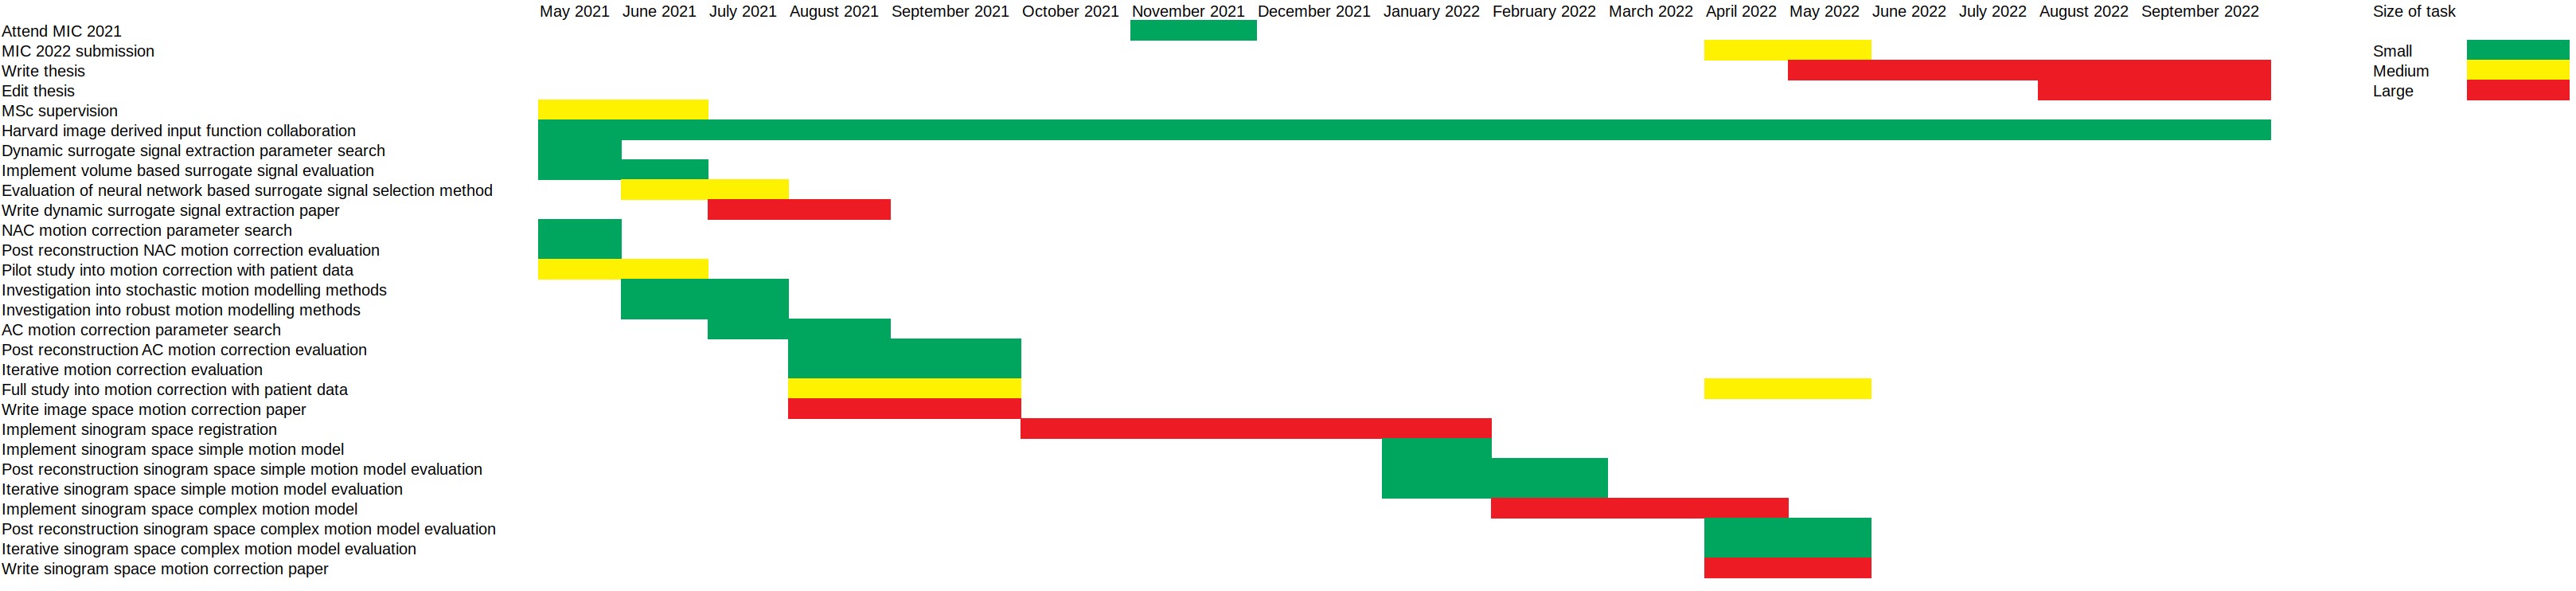
\includegraphics[width=1.0\linewidth]{figures/future_work_gantt_chart.png}
                    
                \captionsetup{singlelinecheck=false, justification=centering}
                \caption{This figure shows a Gantt chart broken up into months from May $2021$ until September $2022$. The tasks which are currently foreseen are broken up into rows and the box under the months in which each activity is expected to take place in is coloured in green.}
                \label{fig:future_work_gantt_chart}
            \end{figure}
        \end{landscape}
        
        The following subsections will address future work which will be performed. The subsections follow on from a more general discussion of future work in each of the previous chapters, which can be found here~\Fref{sec:impact_of_tof_on_respiratory_motion_model_estimation_using_pre_gated_no_intra_cycle_motion_nac_pet_conclusion}, here~\Fref{sec:pet_ct_respiratory_motion_correction_with_a_single_attenuation_map_using_nac_derived_deformation_fields_conclusion},
        here~\Fref{sec:comparison_of_motion_correction_methods_incorporating_motion_modelling_for_pet/ct_using_a_single_breath_hold_attenuation_map_conclusions}, here~\Fref{sec:impact_of_tof_on_respiratory_motion_model_estimation_using_nac_pet_discussion} and here~\Fref{sec:pca_data_driven_surrogate_signal_extraction_methods_for_dynamic_pet_discussion_and_conclusion}.
        
        There are two main aspects to the work which has taken place so far and most probably to the work which will take place prior to the final thesis. These two aspects are respiratory \gls{MC} using \glss{MM} and dynamic \gls{SS} extraction. From the discussions seen in~\Fref{sec:impact_of_tof_on_respiratory_motion_model_estimation_using_nac_pet_discussion} and~\Fref{sec:pca_data_driven_surrogate_signal_extraction_methods_for_dynamic_pet_discussion_and_conclusion} there are a number of directions in which the work could go. The following will discus these directions before solidifying the more general direction in which it is most likely to go (providing time requirements).
        
        \begin{itemize}
            \item As discussed in~\Fref{sec:impact_of_tof_on_respiratory_motion_model_estimation_using_nac_pet_discussion} the methods presented suffer from a number of issues. Firstly, an obvious hole in the results presented above is that the method has only been tested on simulated data. An additional issue posed by the use of \gls{XCAT} simulations would be that the \gls{MM} used to drive the simulation over time is rather simple, it is a linear \gls{MM}.
            
            Furthermore, the objective function used for the \gls{MM} fitting used \gls{SSD} which is sensitive to outliers. A final limitation would be that the objective function for the registration is currently calculated in image space.
            
            As indicated by the results in~\boxcite{Bousse2016a} and~\boxcite{Bousse2016b}, it could be advantageous to perform \gls{MC} using an objective function calculated in sinogram space for a number of reasons, including that the \gls{TOF} sinogram inherently contains more information than the reconstructed volume as well as that if a sinogram space objective function was used it would unify the space in which the \gls{PET} reconstruction and \gls{MC} would be working in. Furthermore, it would be more likely that at early iterations of an iterative \gls{PET} reconstruction and \gls{MC} method that the \gls{MC} would find more usable results rather than steering both optimisations in the wrong direction, this is because the gradient would be being calculated with respect to the measured data.
            
            Thus it appears from above that there are three main issues that need to be tackled. Firstly, there is the issue of testing the method on either more complex simulation data or there is the issue of testing the method on patient data, it would be more interesting as well as provide more useful results to test the method on patient data.
            
            Secondly, there is the issue of robust \glss{MM}, to mitigate the issues of using \gls{SSD} to fit the \gls{MM} an objective function which is robust to outliers could be used, such as Huber. Huber is defined as being equivalent to squared error below a threshold and absolute error above it. Alternatively \gls{RANSAC}, where the \gls{MM} would be fit on different subsets of the data where outliers are removed, or performing the regression on the result of \gls{PCA} on the \glss{DVF} could be investigated.
            
            Finally, there is the issue of implementing a sinogram space objective function for \gls{MC}. A sinogram space objective function for \gls{PET} \gls{MC} has been used previously in~\boxcite{Bousse2016a} and~\boxcite{Bousse2016b}. The most reliable way to implement this would probably be to initially implement an \gls{IR} method which takes (potentially \gls{2D}) volumes and directly registers them together (in other words the \gls{DVF} is not parameterised) with an objective and gradient function calculated on the forward projection of these volumes. This would allow for full testing of the objective and gradient functions in a simple and quick environment. Taking this method and expanding it with a B-spline parameterisation of the \glss{DVF}, a regularisation term (such as \gls{BE}) and using \gls{3D} volumes should be simple and each addition can be independently tested and evaluated. Furthermore, the \glss{MM} used in~\Fref{sec:comparison_of_motion_correction_methods_incorporating_motion_modelling_for_pet/ct_using_a_single_breath_hold_attenuation_map} can be applied directly on top of this method. Once these steps have been taken it can be safe to assume that the sinogram space objective and gradient functions will be well tested and evaluated, at this point it would be possible to transplant them into other code (for instance, code which directly fits the \gls{MM} on the input data without requiring a registration step).
            
            \item As discussed in~\Fref{sec:pca_data_driven_surrogate_signal_extraction_methods_for_dynamic_pet_discussion_and_conclusion} the work on the extraction of a respiratory surrogate signal from dynamic PET data presented previously suffers from a few limitations. Firstly the method has not been tested to \gls{MC} data, it has only been evaluated by looking at the \gls{SS}. An additional concern is that the method could fail for patients who exhibit abnormal breathing patterns.
            
            In order to \gls{MC} dynamic data it is important to address the issue of the aorta. At the beginning of the dynamic acquisition the radiotracer is concentrated entirely in blood, there is a large pool of this blood in the aorta during the first minute of the scan (tapering off over this minute). This large, highly active region can cause issues with \gls{MC}. Thus, to test the dynamic \gls{SS} extraction method in this domain it would be important to either ignore this part of the acquisition or to find a way to extrapolate \gls{MC} to this data without fitting the \gls{MC} on this data. This problem could be easily solved by incorporating \glss{MM}, if a \gls{MM} were fit on data after the point where the aorta dominates the \gls{FOV} then it could be used in collaboration with the \gls{SS} to generate \glss{DVF} for this data regardless. Another method which could be developed to enhance the method would be to introduce machine learning. A \gls{NN} could be added to replace the three window method of selecting and combining \glss{PC}, a \gls{NN} could be trained to identify signals which are caused by respiration.
        \end{itemize}
        
        In more detail and for a breakdown of the time allocated to completing the following work please see the Gantt chart provided here~\Fref{fig:future_work_gantt_chart}. A breakdown of individual tasks extrapolated from the high level tasks is to follow.
        
        \subsection{Motion Correction} \label{sec:future_work_motion_correction}
            The following is specifically related to the future work to complete the bulk of what is required for the \gls{MC} portion of the thesis and expands upon and clarifies what was discussed specifically in~\Fref{sec:impact_of_tof_on_respiratory_motion_model_estimation_using_pre_gated_no_intra_cycle_motion_nac_pet_conclusion}, in~\Fref{sec:pet_ct_respiratory_motion_correction_with_a_single_attenuation_map_using_nac_derived_deformation_fields_conclusion}, and here~\Fref{sec:impact_of_tof_on_respiratory_motion_model_estimation_using_nac_pet_discussion}.
            
            \begin{itemize}
                \item \gls{NAC} \gls{MC} parameter search: This work further optimisation from the work submitted to MIC $2021$, as will be discussed further in~\Fref{sec:future_work_conferences_and_papers}. Currently pair-wise and group-wise methods to \gls{MC} very noisy \gls{NAC} \gls{PET} data have been implemented, both with and without a \gls{LR} based \gls{MM} (from here on referred to as a simple \gls{MM}). However, good parameters to best demonstrate each method have not yet been found. In order to find good parameters simulations such as those presented in~\Fref{sec:pet_ct_respiratory_motion_correction_with_a_single_attenuation_map_using_nac_derived_deformation_fields} have been created and a grid search must be performed, using each method.
    
                \item Post reconstruction \gls{NAC} \gls{MC} evaluation: This section of work is specifically related to taking the parameters found from the previous step and using them in, combination with each relevant method, to generate results. Then, these results must be evaluated using methods such as examining a profile across a lesion inserted into the simulation data, as well as generating pseudo \gls{SUV} and ideally tracking the result of applying the \glss{DVF} generated only to the lesion, in isolation, to establish the quality of the motion captured. These evaluation metrics have all been mentioned before in~\Fref{sec:impact_of_tof_on_respiratory_motion_model_estimation_using_nac_pet}.
    
                \item Pilot study into \gls{MC} with patient data: It is an important milestone for the work in general to test it on patient data, as this will be the most difficult environment for it and will lead a lot of credibility, more so than testing on simulations. Because a \gls{GT} does not exist for patient data it will be a lot more difficult to evaluate, however, similar methods to those employed previously can still be used. For instance, a profile across the diaphragm can show how well gates are registered together, the greater the intensity of the diaphragm and the sharper the drop in intensity going into the lung the better. Additionally, \gls{SUV} are often used as a measure of the accuracy of \gls{MC}, the higher the value in a given \gls{ROI} the better. Furthermore, all methods of calculating \gls{SUV} from the literature have already been implemented.
    
                \item Investigation into stochastic \gls{MM} methods: As mentioned in~\Fref{sec:impact_of_tof_on_respiratory_motion_model_estimation_using_nac_pet_discussion} at this point there should be time to investigate the effects of implementing a stochastic-like \gls{MM} based \gls{MC} method. This could mean either updating the target volume more frequently than at the end of every iteration (for instance updating the target volume after a subset of the data to speed up convergence) or using a subset of the data at each iteration and extrapolating \glss{DVF} for unseen data in the \gls{MC} using the \gls{MM} and \gls{SS} values of the unseen data. These methods could be considered to be similar in a way to the updates proposed to \gls{MLEM} by \gls{OSEM} and may provide similar benefits.
    
                \item Investigation into robust \gls{MM} methods: as mentioned in~\Fref{sec:impact_of_tof_on_respiratory_motion_model_estimation_using_nac_pet_discussion} it may be beneficial to investigate robust \gls{MM} methods. It has been observed that the simple \gls{LR} based \gls{MM} methods used currently do not fit the input data well, this could be because either the input data is very noisy (and the \gls{MM} is helping to smooth this) or the \gls{MM} is not able to fit the data well due to outliers affecting the result. Additionally, the effect seen could be a combination of the two hypotheses mentioned previously. Thus to see which is the case a study into the impact of robust regression methods could be employed here. If results are improved by robust regression then results are better, which is always appreciated, if results are degraded then it lends evidence to the \gls{MM} methods excellent noise suppression capabilities. Robust regression methods which could be tested include the Huber objective function for a \gls{SGD} based regression or \gls{RANSAC}. Furthermore, applying \gls{PCA} to the \glss{DVF}, thresholding a percentage of the least significant \glss{PC} and fitting the \gls{MM} on the resulting eigenvectors before reconstructing the initial \glss{DVF} has proven to give good results when tested on \gls{CT}~\boxcite{Li2011a}~\boxcite{Staub2011}~\boxcite{Chetvertkov2016PrincipalPatients}. Thus it seems appealing to test its validity on \gls{PET} data too.
    
                \item \gls{AC} \gls{MC} parameter search: Although it may be possible to apply the method above to \gls{AC} data using the parameters from the \gls{NAC} based parameter search. It would be ideal to do a further parameter search on \gls{AC} data due to the significant differences in expectation for both and the possibility of significantly improved results.
    
                \item Post reconstruction \gls{AC} \gls{MC} evaluation: This step involves applying the same evaluation steps mentioned previously but this time on \gls{AC} data, using the parameters from the previous section. 
    
                \item Iterative \gls{MC} evaluation: Here the method will be expanded to iterating between \gls{MC} and reconstruction. It has been shown previously, in other work, that there are advantages to interleaving the two processes, as seen in~\Fref{sec:applying_motion_correction}. For instance, the quality of both the accuracy of the \gls{MC} and reconstruction can mutually benefit. However, here the objective function of the \gls{MC} method is based on the comparison of images rather than the sinograms directly, thus the \gls{MC} could struggle to give sensible results for the first few iterations and as such may cause the reconstruction not to converge or to converge slowly. Obviously, weighting and tolerance methods can be employed to reduce the number of iterations of the \gls{MC} method at early time points, however it could be more advantageous to simply change the objective function of the \gls{MC}. It may also be interesting at this point to assess the number of \gls{NAC} and \gls{AC} iterations of both the \gls{MC} and reconstruction to minimise the artefacts associated with a misaligned \gls{Mu-Map} while also trying to minimise overall computation time (obviously as more iterations of both parts of the method are applied the error will reduce but it is to be expected that after a certain point there will be diminishing returns).
    
                \item Full study into \gls{MC} with patient data: At this point it makes most sense to apply it to patient data and evaluate it for the paper which should be written on this work. Additionally, later once the sinogram space based methods are implemented another comprehensive evaluation of the new method will take place using patient data.
    
                \item Implement sinogram space registration: This piece of work entails writing an optimisation method which can register two volumes to each other using an objective function and gradient function which are calculated by comparing the forward projection of those volumes. It is most likely that initially this registration framework will be an asymmetric registration method performing a direct non-parametric registration. In other words the registration would be different depending on which volume is the reference and which is the floating volume and the optimisation will directly find the \gls{DVF} for each registration. Once this has been achieved it would make most sense to attempt to adapt the code to perform parameterised registrations where a B-spline \gls{CPG} is optimised for, this would be consistent with the registration software currently used. Additionally, regularisation terms should be added, such as bending energy which penalises large fluctuations in neighbouring deformations. Taking control of the registration code offers additional advancements not currently available, for instance the current software used cannot be initialised with a \gls{DVF} thus all registration iterations start from scratch significantly increasing computation time.
    
                \item Implement sinogram space simple \gls{MM}: Once the sinogram space registration package is implemented it should be trivial to add the simple \gls{MM} code on top, it is simply a \gls{LR} between the resulting \gls{DVF} and already existing \gls{SS}. However, an additional advantage of taking control of the registration is that the B-spline \gls{CPG} can be output along with the \gls{DVF} and the \gls{MM} could be built using either. It should be more computationally efficient to fit the \gls{MM} on the B-spline \gls{CPG} coefficients without impacting accuracy.
    
                \item Post reconstruction sinogram space simple \gls{MM} evaluation: As previously this means to evaluate the sinogram space based \gls{MC} method both with and without using a \gls{MM} on \gls{NAC} and \gls{AC} data. The evaluation will most likely take place using the same metrics as before and the results should be compared to the image space results.
    
                \item Iterative sinogram space simple \gls{MM} evaluation: The code should already exist at this point to immediately from the previous step begin testing the sinogram space \gls{MC} methods iteratively with reconstruction. For the previous work to be successful it would be expected that the results at this point show a significant improvement over using the image space \gls{MC} methods iteratively with reconstruction.
    
                \item Implement sinogram space complex \gls{MM}: This would be quite a complex piece of work and as of yet it is difficult to say how it would be achieved. The aim would be to combine the work from~\boxcite{McClelland2017} with the sinogram space based \gls{MC} method to allow for a \gls{MM} to be fit directly on the input data without doing a separate registration and \gls{MM} fitting step. Taking the objective function from the sinogram space \gls{MC} method and combining the gradient function with that of~\boxcite{McClelland2017} using the chain rule should allow for this to be possible. However, it's always much easier said than done. This is the end goal of the work to make this achievable.
    
                \item Post reconstruction sinogram space complex \gls{MM} evaluation: Again, take the evaluation methods mentioned previously, however, this time apply it to the results from the 'complex' \gls{MM} work (in other words the direct fitting of the \gls{MM} on the input data from the previous step). This should be applied on patient data, as mentioned previously.
    
                \item Iterative sinogram space complex \gls{MM} evaluation: Finally this brings together everything mentioned previously, this is a comparison and evaluation of the complex \gls{MM} method applied to patient data with the simple \gls{MM} method.
            \end{itemize}
        
        \subsection{Dynamic Data Driven Surrogate Signal Extraction} \label{sec:future_work_dynamic_data_driven_surrogate_signal_extraction}
            The following is specifically related to the future work to complete the tangential work performed in the domain of dynamic \gls{DD} \gls{SS} extraction and expands up and clarifies what was discussed specifically here~\Fref{sec:pca_data_driven_surrogate_signal_extraction_methods_for_dynamic_pet_discussion_and_conclusion}.
            
            \begin{itemize}
                \item Dynamic \gls{SS} extraction parameter search: Values of parameters were initially selected to validate the efficacy of the underlying assumptions of the method. Now that it has been proven that those assumptions were not entirely wrong, new parameters must be found for the dynamic \gls{SS} extraction methods which are generalisable to the entire data set. This process involves running all possible combinations of the method with a subset of the data and trying different combinations of possible parameters in a logical manner, keeping the best result each time. It has been found that the method is sensitive to the selection of parameters and as such it is an important step to find the best results. However, because of the time taken for each execution and because now testing each parameter means running the method with multiple data sets, this is a very time consuming process.
    
                \item Implement volume based \gls{SS} evaluation: Currently, the collection of dynamic \gls{SS} extraction methods are only evaluated using metrics which are calculated based on the signal itself directly. Because an important use case of this work would be to \gls{MC} dynamic \gls{PET} data, such as by methods like those discussed in~\Fref{sec:impact_of_tof_on_respiratory_motion_model_estimation_using_nac_pet}, it would be beneficial to also evaluate the result of doing this using the \glss{SS} generated here. For instance, \gls{MC} could be applied, first on late time point data and then extrapolating to early time point data to avoid issues related to the aorta (thus being another application of \gls{MM}, for the extrapolation), before being evaluated by looking at profiles of the data and \gls{SUV}.
    
                \item Evaluation of \gls{NN} based \gls{SS} selection method: Following on from the discussion in~\Fref{sec:pca_data_driven_surrogate_signal_extraction_methods_for_dynamic_pet_discussion_and_conclusion} a \gls{NN} based method to discriminate between signals which reflect good respiratory \gls{SS} and those which do not has recently been made available. It would be a positive piece of research, and also quick to implement, to test the select and combined method, presented in~\Fref{sec:pca_data_driven_surrogate_signal_extraction_methods_for_dynamic_pet_methods_selecting_and_combining_pcs} but by replacing the frequency window discrimination method with the \gls{NN} based method.
            \end{itemize}
        
        \subsection{Conferences and Papers} \label{sec:future_work_conferences_and_papers}
            The following is a quick breakdown of the conferences which work will be submitted to as a minimum and otherwise the papers which could feasibly be written regarding the future work.
            
            \begin{itemize}
                \item Attend \gls{MIC} $2021$: Provided that the submitted work is accepted then time will be allocated to attending the \gls{MIC} in $2021$.
    
                \item \gls{MIC} $2022$ submission: The intention is to continue as before with submitting work to the \gls{MIC} each year. As of yet it is not possible to say what will be submitted to the \gls{MIC} in $2022$, however it is safe to say that as long as work goes as expected with \gls{MSc} Supervision, as seen in~\Fref{sec:future_work_miscellaneous}, that it would be possible to submit this along with any work performed after the $2021$ deadline. The date of the conference itself is beyond the forecast of this section, however it is always positive to increase the number of quality publications regardless of other factors.
                
                \item Write dynamic \gls{SS} extraction paper: Thus far it appears that there could be enough material from the dynamic \gls{SS} extraction work to warrant a full paper submission to a relevant journal, this is especially true if the additional work suggested in~\Fref{sec:future_work_dynamic_data_driven_surrogate_signal_extraction} is completed in a timely manner and with positive results. Similar papers have been published previously with roughly equivalent results so this doesn't seem unreasonable~\boxcite{Schleyer2014}~\boxcite{Kesner2010AMethods}.
                
                \item Write image space \gls{MC} paper: This is the minimum achievable goal, if no other paper is submitted or accepted at least this one must be in order for the work be considered successful at all. This paper should contain the work expressed in~\Fref{sec:impact_of_tof_on_respiratory_motion_model_estimation_using_nac_pet} plus the work which is planned to be submitted to \gls{MIC} $2021$ plus the advancements mentioned in~\Fref{sec:future_work_motion_correction} which are focused solely on registrations taking place where their objective function is in image space. This can still include iterative \gls{MC} methods as well as being applied to patient data, ideally.
                
                \item Write sinogram space \gls{MC} paper: This is the ideal goal, as well as the paper mentioned above the main aim of future work is to extend to performing \gls{MC} using a registration method with an objective function calculated directly on the sinograms, rather than the reconstructed volumes. This should provide better results faster than with an image space based metric (faster in the sense of the total number of iterations rather than temporally), as well as meaning that the objective function of both the registration method and reconstruction would be using objective functions in the same space.
                
                \item Write thesis: It may be wishful thinking to assume that six months is adequate to complete this in, however a lot of what is written here can be used in the thesis. Regardless it is likely that the thesis will be updated incrementally as work is performed before the allocated time in the Gantt chart above in~\Fref{fig:future_work_gantt_chart}.
    
                \item Edit thesis: Realistically editing of the thesis should be an ongoing process throughout the writing phase. However, this is here as a buffer at the end of the writing process specifically to address comments on drafts of the thesis as well as to allow the writing process itself to overflow, if it must, slightly.
            \end{itemize}
        
        \subsection{Miscellaneous} \label{sec:future_work_miscellaneous}
            The following are miscellaneous activities which are intended to be carried out along the way or simultaneously of performing the above.
            \begin{itemize}
                \item \gls{MSc} supervision: There is an \gls{MSc} student working on continuing previous work into \gls{SS} extraction directly using a \gls{NN}. Ideally if this work proves fruitful then it would seem logical to attempt to adapt the work to rival the more traditional approaches presented previously to extract \gls{SS} from dynamic data. A brief description of the methodology is as follows, train an autoencoder to reduce the dimensionality of the input sinograms to a sufficiently low level in the latent layer, this can be trained unsupervised on all sinograms available. Next a network will take the latent layer variables and learn to combine them in such a way to lead to the desired output. This method is similar to the method presented in~\Fref{sec:pca_data_driven_surrogate_signal_extraction_methods_for_Dynamic_pet}, however the autoencoder replaces \gls{PCA} and the network to combine latent layer variables replaces the select and combine procedure.
    
                \item Harvard image derived input function collaboration: There is an ongoing collaboration with Harvard which intends to use a similar \gls{NN} based method to that one presented above, however replacing the input with dynamic reconstructions and replacing the output with the blood curve required for kinetic modelling.
            \end{itemize}
